\documentclass{article}
\usepackage[utf8]{inputenc}
\usepackage{amsmath}
\usepackage{hyperref}
\usepackage{xcolor}
\usepackage{graphicx}
\usepackage{minted}

\setminted[python]{breaklines, framesep=2mm, fontsize=\footnotesize, numbersep=5pt}

\title{ASTR 305 \\ Problem Set 3}
\author{Avichal Kaul}
\date{23 September 2022}
% Please give me extra credit for doing this in latex :p

\begin{document}

\maketitle

\section{Problem 1}

\subsection{The Problem}
We can start by changing variables for the Planck Function integral. Here is the original equation:
\begin{equation}\label{eq:1}
    \sigma T^{4} = \pi \int_{0}^{\infty}B_{\nu}(T) d\nu
\end{equation}
The LHS requires no modification right now. Let's deal with the Planck function by taking $\frac{h\nu}{kT} = x$.
\begin{gather*}
    \nu = x\frac{kT}{h}\\
    d\nu = \frac{kT}{h}dx
\end{gather*}
We plug Planck's function and our values into \ref{eq:1}.
\begin{equation}\label{eq:2}
    \sigma T^{4} = \frac{2\pi}{c^2} \frac{(kT)^4}{h^3} \int_{0}^{\infty}\frac{x^{3}}{e^{x}-1}dx
\end{equation}
Note how the temperature terms already cancel. Now, let's focus on our integral. 
\begin{equation}\label{eq:3}
    \int_{0}^{\infty}\frac{x^{3}}{e^{x}-1}dx
\end{equation}

The integrand has a peak at $x=1$, after which it falls off rapidly in either direction. 

Our integration limits are problematic. They start at $x=0$, at which point the function is undefined, and extend all the way to infinity, where it is impossible to evaluate.

While evaluating the integral from $x=0$ to $x=1$ is certainly easier than evaluating it from $x=1$ to infinity, the singularity at $x=0$ presents a hurdle. We can get around this by finding the limit of the function at this point, and considering that limit the canonical value of the function. In the code, the function implementation contains a check for whether the input is zero: in that case, it returns the limit of the function at zero, which is (also) zero.

The contribution of terms to the integral falls off rapidly as the function increases. Since we know the analytical solution, we can actually estimate this rate of fall off. This is done in figure \ref{fig:1}. Terms greater than or equal to 10 contribute approx. 1/100th of the value of the total integral ($\sim$0.06 vs $\sim$6). So, if we were to set an upper bound at, say, 100 - above which contributions are vanishingly small - we can say with certainty that the result will be accurate enough for our purposes. 

\begin{figure}
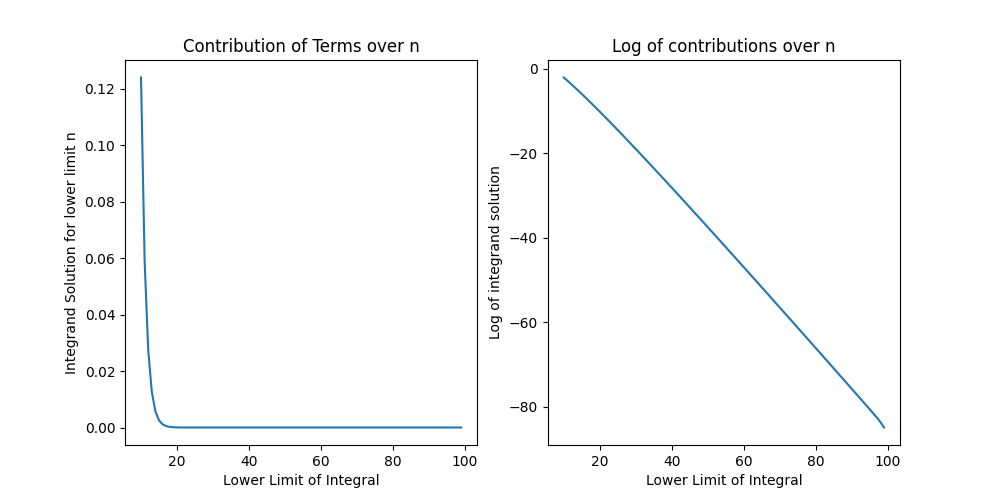
\includegraphics[width=\linewidth]{Figure_2.png}
  \caption{Contributions over lower limit n}
  \label{fig:1}
\end{figure}

\subsection{The Analytical Solution}
As previously mentioned, we know the analytical solution for our integral \ref{eq:3}. 
\begin{equation}
    \int_{0}^{\infty}\frac{x^{3}}{e^{x}-1}dx = \frac{\pi^4}{15}
\end{equation}
We plug this into \ref{eq:2} to get our formula for $\sigma$.
\begin{equation}
    \sigma = \frac{2\pi}{c^2} \frac{k^4}{h^3}\frac{\pi^4}{15}
\end{equation}
Evaluating this gives us roughly $5.67*10^{-5}\frac{erg}{cm^2 K^4 s}$. A more precise solution can be found in the program output.

\subsection{The Programmatical Solution}
Our programmatical solution gave us roughly $5.67*10^{-5}\frac{erg}{cm^2 K^4 s}$, which is a handsome result. Our percentage error was $7.14073*10^{-8}$

\section{Problem 2}
The Gaussian Integral and its integrand are ubiquitous. There's a reason I have them tattooed. The integrand is symmetric about the x axis, which means we can choose a lower/upper bound and set the other bound as the negative of the first.

Alternatively, as a result of this symmetry, we can evaluate the function in only one direction (say, from 0 to +10) and double our result to get the total value of the integral in both directions (from -10 to +10). This is the approach we've decided to use in the programmatic solution, and - interestingly - it seems to be the tiniest bit more accurate. \footnote{Relative error for -10 to 10: 6.4360289102846085e-09. For 2 * 0 to 10: 6.42036010799291e-09}

We can also see how higher term contribution falls off in Figure \ref{fig:boat1}

Here are our outputs. Programmatical Solution! 1.77245E+00. Analytical Solution! 1.77245E+00. Percentage Error! 6.42036E-07%

\begin{figure}
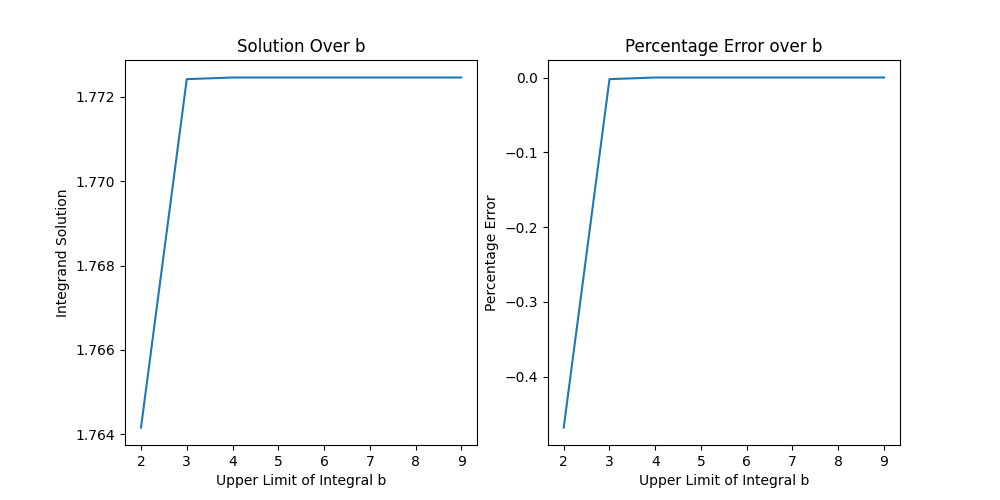
\includegraphics[width=\linewidth]{Figure_1.png}
  \caption{Our results over time.}
  \label{fig:boat1}
\end{figure}

\section{Problem 3}
\subsection{Part (a)}
In the interest of time, I will be copying a lot of the formatting directly from the Gaussian Quadrature Jupyter Notebook. The $n=4$ Gaussian Quadrature looks like this:

$$\tilde I = c_1 f(x_1) + c_2 f(x_2) + c_3 f(x_3) + c_4 f(x_4).$$

where $x_1, x_2, x_3, x_4$ are the roots of the fourth Legendre Polynomial, $P_4(x)$. Let's evaluate these roots.

\begin{gather*}
    P_4(x) = x^4-6x^2/7 +3/35 \\
    x^4-6x^2/7 +3/35 = 0 \\
    x_1, x_2, x_3, x_4 = \sqrt{3/7 - 2/7*\sqrt{6/5}}, -\sqrt{3/7 - 2/7*\sqrt{6/5}}, \\
    \sqrt{3/7 + 2/7*\sqrt{6/5}}, -\sqrt{3/7 + 2/7*\sqrt{6/5}}
\end{gather*}

Using the method outlined in the notebook, we can find the coefficients to be:
\begin{gather*}
    c_1, c_3 = {\frac{18 + \sqrt{30}}{36}} \\
    c_2, c_4 = {\frac{18 - \sqrt{30}}{36}}
\end{gather*}

This expression is exactly accurate upto $2*4-1=7$th degree polynomials.


\begin{figure}
  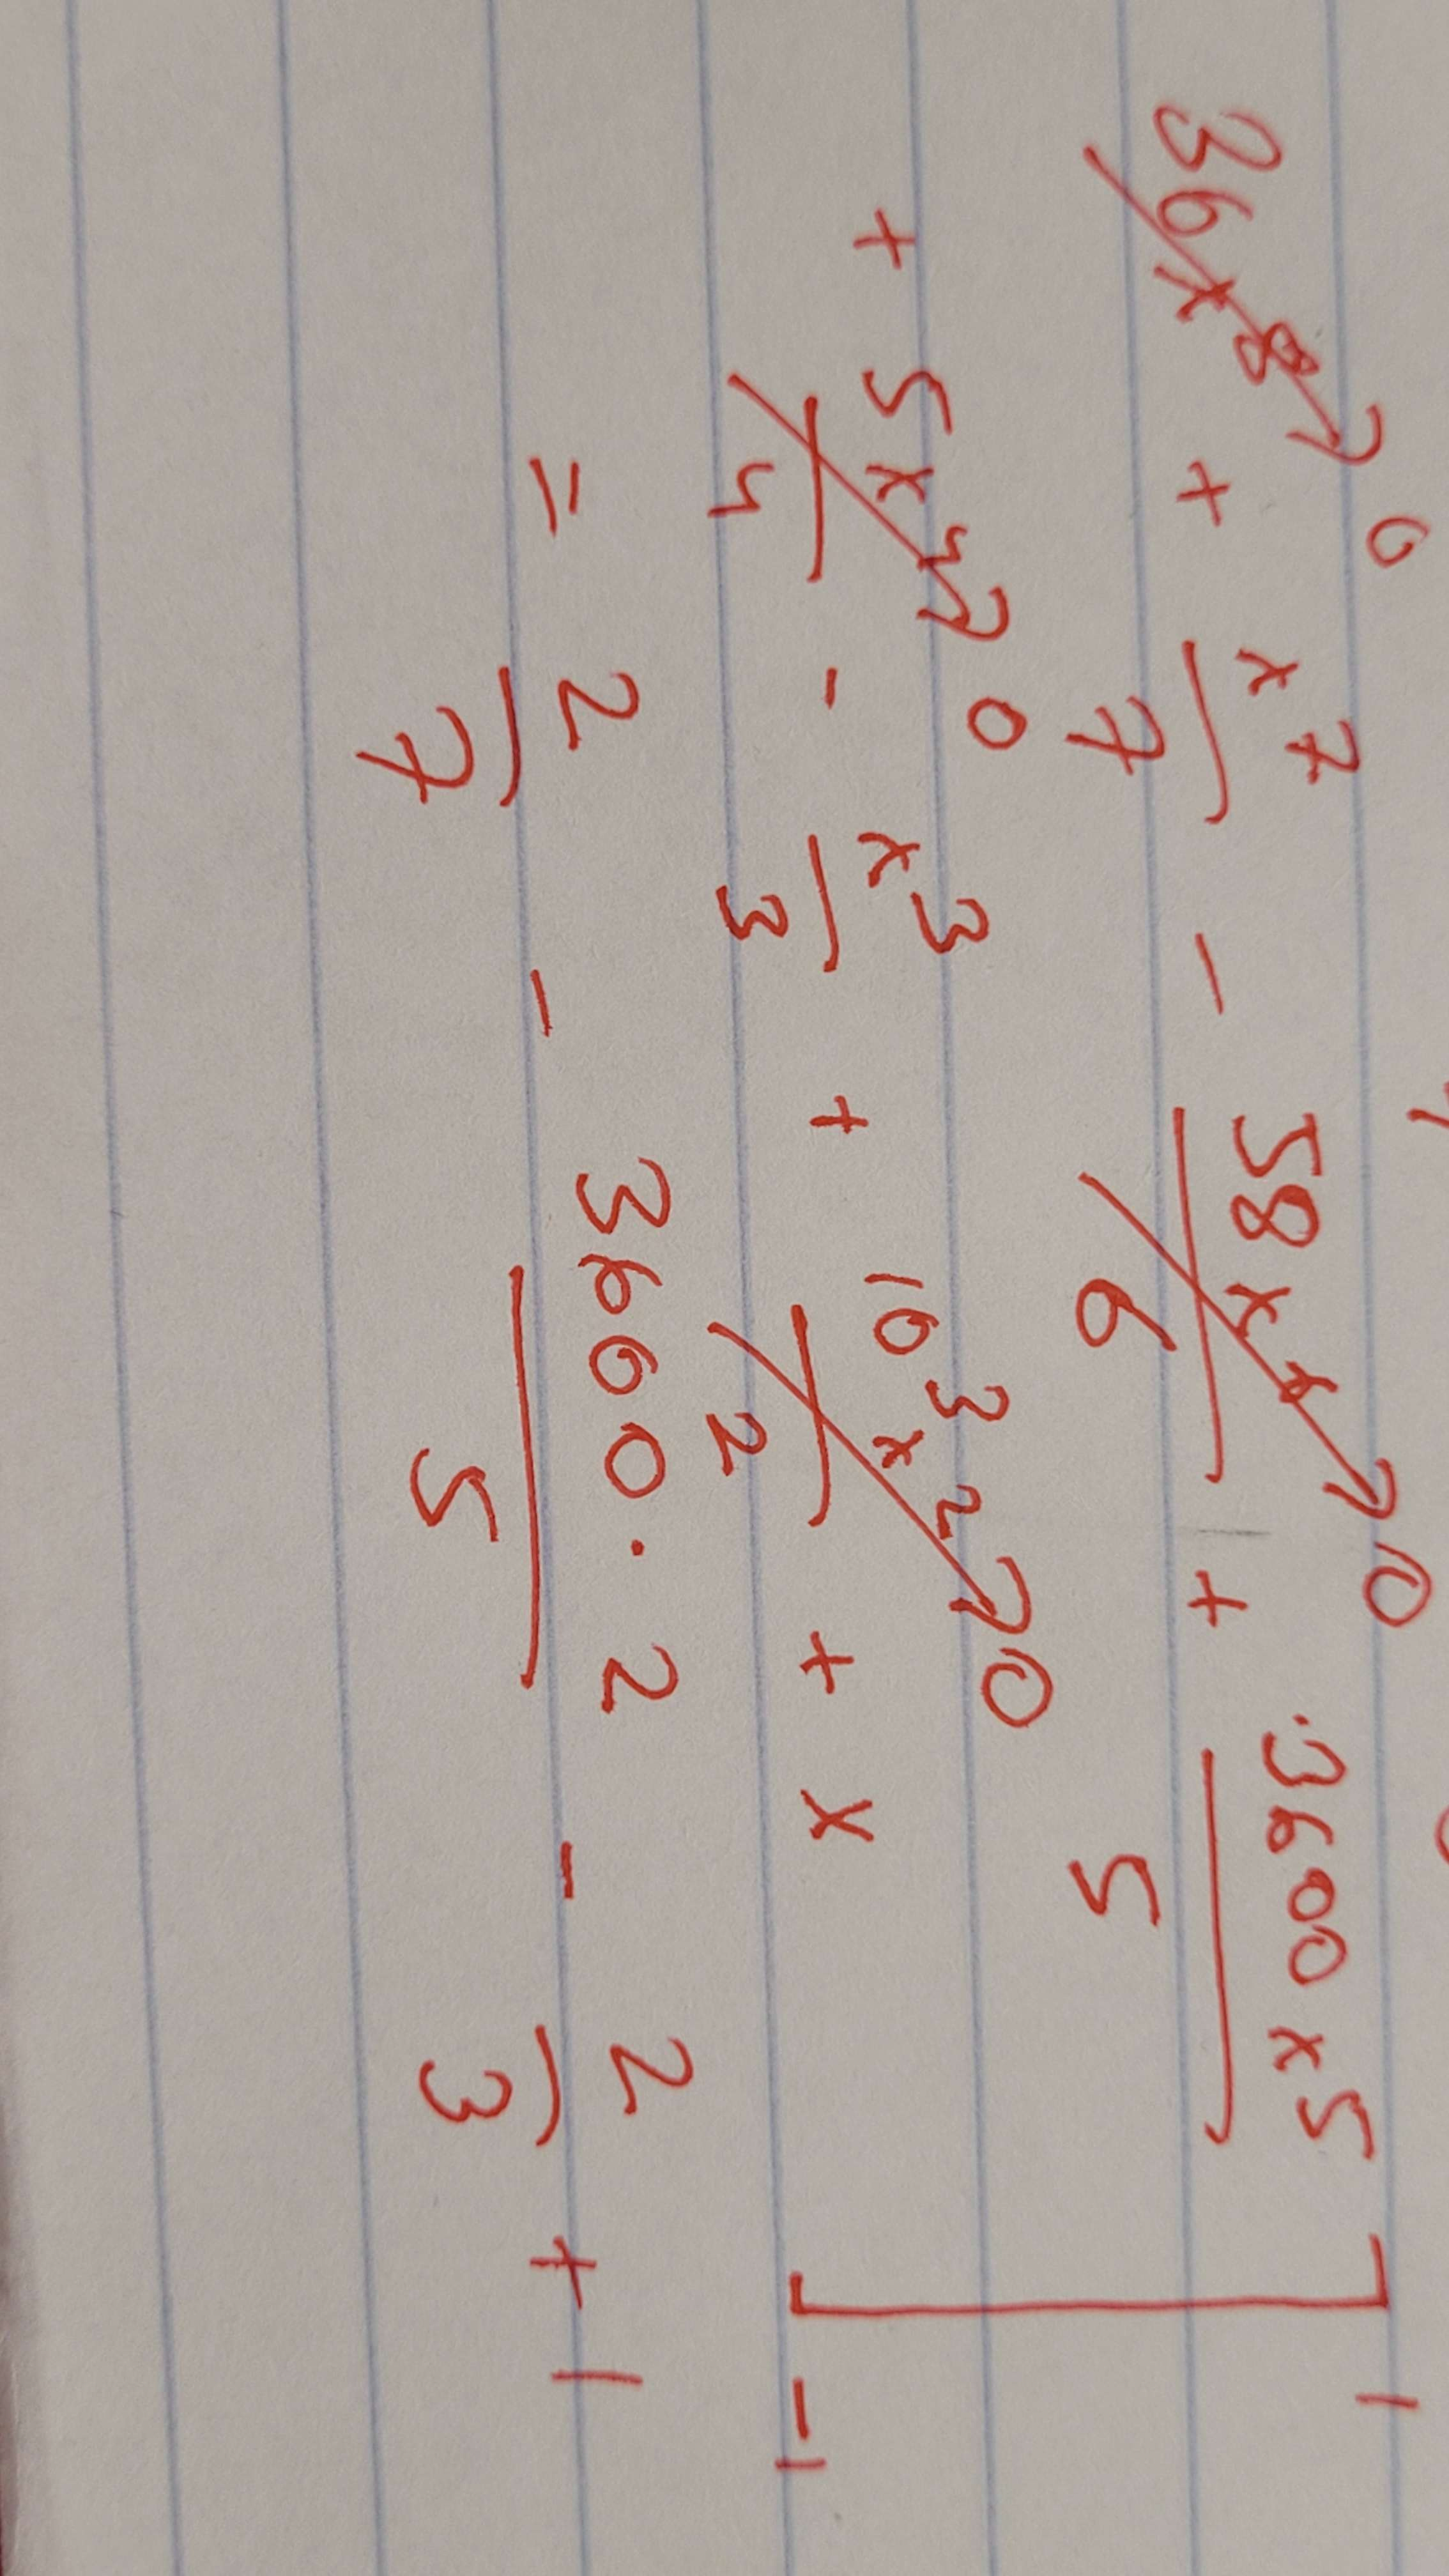
\includegraphics[width=7cm, angle=90]{quick.jpg}
  \caption{Quick and Dirty Analytical Solution}
  \label{fig:ana}
\end{figure}

Analytically, the solution for the provided integral is $2/7-3600*2/5-2/3+1$ (shown in \ref{fig:ana}), or approx. $-1439.38$. We can evaluate the integral using the code in Appendix \ref{appendix:a}. Since our numerical error is on the order of 1e-4\footnote{0.0006947431104646284}, we can confidently say that our Gaussian Quadrature solution agrees with our analytical solution.

\subsection{Part (b)}
To evaluate this, we can use the same Jupyter Notebook with all our Quadrature Models. The code is in Appendix \ref{appendix:b}. 

\begin{gather*}
n = 2 : 0.12197520127865058 \\
n = 3 : 0.0040611225242603854 \\
n = 4 : 6.212054090215524*10^{-05}
\end{gather*}

We note that the relative error for n=4 is two orders of magnitude smaller than that for n=3, and four orders smaller than that for n=2.
Plotting these results in Figure \ref{fig:4}, we find that the error does indeed converge to zero as n increases.

\begin{figure}
  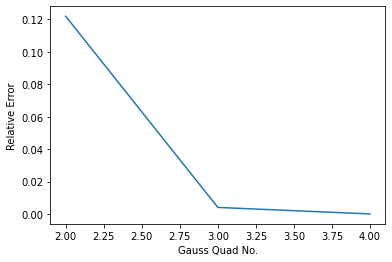
\includegraphics[width=\textwidth]{index.png}
  \caption{Gaussian Quadrature Error Convergence}
  \label{fig:4}
\end{figure}

\appendix
\section{Code Appendices}
\subsection{Problem 3 Part (a) Raw Code}\label{appendix:a}

\begin{minted}[linenos]{python}

def GaussianQ_n4_any_interval(f,a,b,*P):
    n = 4
    #define nodes on [-1,1] interval(derived above)
    t = np.array([np.sqrt((3/7 - 2/7*np.sqrt(6/5))), -np.sqrt((3/7 - 2/7*np.sqrt(6/5))), \
                 np.sqrt((3/7 + 2/7*np.sqrt(6/5))), -np.sqrt((3/7 + 2/7*np.sqrt(6/5)))])
    #define coefficients (derived above)
    c = np.array([(18 + np.sqrt(30))/36,]*2 + [(18 - np.sqrt(30))/36,] * 2)
    I = 0
    #now sum up the integral based on the n=3 Gaussian Quadrature formula
    for j in range(n):
        I += (b-a)/2.*c[j]*f(transform_variable(t[j],a,b),*P)
    return I
    
def func(x, *P):
    return 36*x**7 + x**6 - 58*x**5 -3600*x**4 + 5*x**3 - x**2 + 1000*x + 1
    
exact_value = 2/7-3600*2/5-2/3+1
print(np.abs((GaussianQ_n4_any_interval(func, -1, 1,)-exact_value)/exact_value))
\end{minted}

\subsection{Problem 3 Part (b) Raw Code}\label{appendix:b}
\begin{minted}[linenos]{python}
exact_value = -2.
print(f'n = 2 : {np.abs((GaussianQ_n2_any_interval(func,0,np.pi,*P)-exact_value)/exact_value)}')
print(f'n = 3 : {np.abs((GaussianQ_n3_any_interval(func,0,np.pi,*P)-exact_value)/exact_value)}')
print(f'n = 4 : {np.abs((GaussianQ_n4_any_interval(func,0,np.pi,*P)-exact_value)/exact_value)}')

arr = [np.abs((GaussianQ_n2_any_interval(func,0,np.pi,*P)-exact_value)/exact_value), np.abs((GaussianQ_n3_any_interval(func,0,np.pi,*P)-exact_value)/exact_value), np.abs((GaussianQ_n4_any_interval(func,0,np.pi,*P)-exact_value)/exact_value)]
import matplotlib.pyplot as plt

plt.plot([2, 3, 4], arr, label="Gaussian Quadrature Convergence")
plt.xlabel('Gauss Quad No.')
plt.ylabel('Relative Error')
plt.show()
\end{minted}
\end{document}
